\chapter{The Array}
\label{chap:array}
\section{Why Arrays}

Since this is a data structures course, I assume that students have had exposure to arrays or array like objects. 
This chapter goes into a bit of a deeper detail that may have been glossed over and introduces the topic in the appropriate language if need be.  
In other words, I assume you know what an array is and that you've used it to solve problems;  writing something like a function to find the average of an array of integers in the language of your choice should be laughably straightforward at this point. However, I don't necessarily assume you know how to use it in Java or Python\footnote{Although we use lists in python}, nor have you ``peeked under the hood,'' so to speak.

There are two other important bits.
The first is I want you to understand how your programming language of choice finds an arbitrary index in an array.
The second is that I want to hammer in the point that \textbf{everything is an object in Java and Python, except they're actually references to objects.}


%\begin{itemize}
%	\item because new language: 
%	Since this is a data structures course, I assumed that students have had exposure to arrays or array like objects.
%	This chapter goes into a bit of a deeper detail that may have been glossed over and Introduces the topic in the appropriate language if need be.
%	
%	In other words, I assume you know what an array is, but not necessarily how to use it in Java or Python\footnote{Although we use lists in python}.
%	\item  Because internal memory lookup
%	\item Because we need to make sure internal knowledge is cohesive (eg arrays of objects are arrays of pointers/references)
%\end{itemize}
%






\section{Java and Arrays}
The Array is a built in class in Java, but the syntax is a bit unique \footnote{Enough so that I constantly had to look up how to do it my first two years of undergraduate studies, so don't feel too bad if you have to do the same.}

To create an array in Java we do:

%\begin{minted}{Java}
%	Type[] myArray = new Type[sizeOfArray]
%\end{minted}
\begin{minted}{Java}
Type[] myArray = new Type[sizeOfArray]
\end{minted}


Here, every item in the array is of whatever \texttt{Type} we want, which could be a Class or primitive.   
Arrays can be whatever integer size we desire, but once set it cannot be changed.
This is because to create an array, the computer allocates a contiguous block of memory.
If we wanted to resize it, there is no guarantee that this chunk of memory won't have things directly before or after it, preventing us from safely extending its range.

This small fact can lead to some fun shenanigans in other programming languages such as C.

\section{Python and Arrays}
\label{sec:python-arrays-lists}
Python doesn't really do arrays in the same way.
It instead uses Lists, as we'll see in Chapter \ref{chap:arraylist}.

The Python code \mintinline{Python3}|myNotArray = []|  does not actually make an array like you assume it would in some other language.  Instead it makes a list (specifically an arraylist) to contain these items.
The syntax works exactly like an array in other languages, but you get access to some nifty operations in Python, like slicing, concatenation, and  built-in methods.  In addition, Python dynamically resizes this array if we need it bigger or smaller.\footnote{We cover the specifics in Chapter \ref{chap:arraylist}}


However, if you really want or need to use an array in python, you can.
%TODO factcheck
There are two ways to accomplish this.
The first way is the built in \texttt{array} package.  This builds a wrapper for the more primitive but efficient C-based array. 
The python package \texttt{numpy} contains yet \textit{another} type of array, this time much more focused on mathematical operations. 
In short, if you're working in python, use a the default list where you would normally use an array unless you know you should use something more specialized.


Regardless, the next sections will still be valuable because an array-based list, like what Python uses, uses an array internally.

\section{How an Array Works}

As previously mentioned, an array creates a contiguous block of memory.  But what does this actually mean?
%autogenerated placeholder diagram  by chatgpt
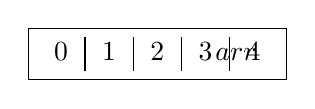
\begin{tikzpicture}
	\node[rectangle, draw] (array) {
		\begin{tabular}{c|c|c|c|c}
			0 & 1 & 2 & 3 & 4 \\
		\end{tabular}
	};
	\node[right of=array] (label) {$arr$};
\end{tikzpicture}

Here, $arr$ does not contain the array; it holds a reference to the array.  The correct term varies on the language you are using, but the point is that $arr$ tells you the location of the array rather than holding the array itself.  Remember, arrays are objects;  any variable holding an object is, in reality, holding the memory location of that object.


\subsection{Operations}

To review, arrays have two operations and one attribute: storing a value at an index, retrieving a value from an index, and their size. 
Interestingly enough, this is one of the few consistent notations across multiple programming languages.
For an array \texttt{arr}, retrieving a value from an array is and storing it in some variable is done with \mintinline{Java}|myVar = arr[index]|.
To store some \texttt{newItem} in \texttt{arr}, you use \mintinline{Java}|arr[index] = newItem|.
Figuring out the length of an array in Java is done with \mintinline{Java}|arr.length|,\footnote{This is one of the little things in Java that can be a source of frustration.  Strings use \texttt{.length()}, arrays use \texttt{.length}, and Collections like Lists and Sets use \texttt{.size()}. I understand why, but I die a little inside every time I have to explain it.}
and in Python, a simple \mintinline{Python3}|len(arr)| works.

%\begin{minted}{Java}
%	int len = arr.length;
%\end{minted}


\subsection{Array Internals and the Memory Formula}
\label{array-formula}

So how does an array actually work?  How do you actually retrieve a value from an index?
The most crucial thing to keep in mind in this textbook is when you see something like the code below:
\begin{minted}{Java}
variable = expression;
\end{minted}

The left side is always a variable.  
The expression on the right side always yields some memory location.\footnote{except for primitives, like \texttt{int} in Java}  
%This means you should repeat to yourself ``the memory location on the right gets stored in the variable on the left.''
This means that \mintinline{Java}|int[] numbers = new int[10]| stores a memory location in \texttt{numbers}.  
It does not store 10 integers in \texttt{numbers}.  It only tells you where to find them.  
Specifically, \texttt{numbers} stores the memory location of index 0 of the array.  
This is true for not only Java, but C as well, and almost every programming language\footnote{Python and other interpreted languages are slightly more complicated because we are dealing with array lists, thus one additional level of abstraction, so this storage just happens a layer deeper.  Esoteric languages like \textit{ook} and \textit{Malbolge}  prevent me from making a statement like ``all languages.''}. 


Thus, the variable that holds the reference to the array is always holding the location of the first index - index 0. In addition, we always know the size of an individual ``slot'' in an array, either because it is an array of primitives or objects(see below).
As a result, our programs can find the memory location of any index of an array using a constant time\footnote{See Chapter \ref{chap:analysis} for that term, but basically, no matter how big the array, an index lookup requires only a single multiplication and addition operation.} lookup using the following formula. 

$$\mathtt{location} = \mathtt{arr} + \mathtt{index} \cdot \mathtt{sizeof(element)}$$

In the above formula, \texttt{arr} is the variable holding the reference to the array, which is the starting memory location. Next, \texttt{index} is the desired index and \texttt{sizeof(element)} is the size (in bytes) of a ``slot''  of \texttt{arr}.


Here's an example.  Suppose we have some arr \texttt{arr}, which is a reference to an array of 64-bit  floating point numbers (\texttt{double} in Java, \texttt{float} in Python\footnote{stings like a C.}). 64-bits is 8 bytes, so each ``slot'' of the array is 8 bytes.  Let's say that \texttt{arr}'s memory location is at address\footnote{When dealing with memory locations/addresses, convention is to use hexadecimal or base 16.  If you're unfamiliar, this just means each digit can have 16 distinct symbols, representing the decimal values 0-15, with A being 10 and F being 15.} 0x0000BEEF, which means index 0 is at 0x0000BEEF. If we want to find index 3, we can plug it into the formula.

\begin{equation} \label{eq:arr-formula}
	\begin{split}
		\mathtt{location} & = \mathtt{arr} + \mathtt{index} \cdot \mathtt{sizeof(element)} \\
		& = \mathtt{0x0000BEEF} + 3 \cdot \mathtt{sizeof(double)} \\
		& = \mathtt{0x0000BEEF} + 3 \cdot 8 \\
		& = \mathtt{0x0000BEEF} + 24 \\
		& = \mathtt{0x0000BEEF} + \mathtt{0x00000018} \\
		& = \mathtt{0x0000BF07}
	\end{split}
\end{equation}


What if we aren't dealing with primitives, but with objects like Strings instead?  
In this case, each slot in the array doesn't hold the object itself but instead \textit{a reference to that object}.
Thus, each slot needs to be big enough to hold a memory address, ie 32 bits or 64 bits depending on the machine and language.





\section{Common Array Algorithms}
Once again, this chapter isn't designed to teach you how to use arrays or how to solve these simple problems.  You have already done that.  I present this problems for a few reasons:
\begin{itemize}
	\item For comparison with Lists in Part \ref{part-list}
	\item You may be learning Java or Python, while knowing the other or neither language.
	\item We will reexamine these problems in the context of runtime analysis.
\end{itemize}

\subsection{Finding Values in an Array}
\subsubsection{Finding the Minimum}

Hopefully you know this one by now!
Simply assume the first item is the smallest item, then check it against every other item in the array.  If an item is smaller that the current smallest item, it replaces the smallest item.

\begin{javacode}[listing and comment, comment={As seen in the comments, it is fairly straightforward to change this code to return the index, rather than the item.}]{Finding the Minimum of An Array}
public static int findMin(int[] arr) {
	int smallest = arr[0];
	// int smallestIndex = 0;
	for (int i = 1; i < arr.length; i++) {
		if(arr[i] < smallest){
			smallest = arr[i];
			// int smallestIndex = i;
		}
	}
	return smallest; // or smallestIndex
}
\end{javacode}

\begin{pycode}[listing and comment, comment={Realistically, just use \mintinline{Python3}|min(arr)|. If you want to find the index, loop thru using \mintinline{Python3}|enumerate|.}  ]{Finding the Minimum of An Array 2}
def findMin(arr):
	smallest = arr[0]
	for num in arr:
		if num < smallest:
			smallest = num
	return smallest
\end{pycode}


\subsubsection{Finding the Average}
Another common problem.  Sum up all the numbers and divide that by how many numbers there were.


\begin{javacode}{Finding the Average in Java}
public static double getAverage(int[] arr) {
	int total = 0;
	for(int num : arr) {
		total += num;
	}
	return ((double) total)/arr.length;
}
\end{javacode}

\begin{pycode}[listing and comment, comment={Or just \mintinline{Python3}|sum(nums)/len(nums)| for a one liner and impress your classmates with how little code you write.}  ]{Finding the Average in Python}
def getAverage(nums):
	total = 0
	for num in nums:
		total += num
	return total/len(nums)	
\end{pycode}



\subsection{Limitations}
Arrays are awesome solutions for many problems, but they are lacking in ability for some problems.  Consider the following exercise:

\begin{verbatim}
Given a string of text, determine what the most common character of text is. 	
\end{verbatim}
Unless you've seen this problem before, there is no obvious solution.
Considerable thought eventually lands on an idea: characters are just integers, so we could assign each one of the characters an index and increment the index each time we see the character.

\begin{javacode}[listing and comment, comment={If this code is a complete mystery to you, that's okay; this conversion is a bit niche.    Every \texttt{char} is actually an \texttt{int} in disguise. You can read up a little on ASCII and Unicode and then do the following two things.  First,  try running \mintinline{Java}|System.out.println((int) 'a');|.  Casting the \texttt{char 'a'} to an \texttt{int} gives us the ASCII value 97.  We can even do some math with this. Next, try running the code \mintinline{Java}|int what = 'b' - 'a';| and print out the value.  You'll get 1, which makes sense, since \texttt{b} is one letter after \texttt{a}. \newline \\  Now that we have established every \texttt{char} has an \texttt{int} value, our code uses this to create an array where the index is the ASCII value of a the character with that \texttt{int} value and the \texttt{int} stored in that slot is the number of times we've seen that \texttt{char} so far.}] {Most Frequent ASCII Character}
public static char mostFrequent(String text) {
	int[] tally = new int[128]; 
	for(char c : text.toCharArray()) {
		tally[(int) c] += 1;
	}
	
	indexWithHighest = 0;
	for(int index = 0; index<128; index++) {
		if( tally[index] > tally[indexWithHighest]){
			indexWithHighest = index;
		}
	}
	return (char) indexWithHighest;
}

\end{javacode}

%TODO: Finish explaination
\begin{pycode}[listing and comment, comment={As above in the Java block, if this code is a complete mystery to you, that's okay; Every glyph is actually an \texttt{int} in disguise. You can read up a little on ASCII and Unicode and then play around with \texttt{ord} and \texttt{chr}.} ] {Most Frequent ASCII Character}
def mostFrequent(text):
	tally = [0]*128 
	for letter in text:
		# https://docs.python.org/3/library/functions.html#ord
		tally[ord(letter)] += 1
	
	indexWithHighest = 0
	for index, count in enumerate(tally): 
		if index> indexWithHighest:
			indexWithHighest = index
			
	return chr(indexWithHighest) # builtin, reverse of ord
}

\end{pycode}


However, this has some serious limitations.  For one, this breaks if we are not using ascii.  What if the text is ``こんにちは'' or other non-english text? 
You could create a larger array for all 100000+ unicode characters, but this begins to become less and less feasible.  
And now what if we change the problem to:

\begin{verbatim}Given a string of text, determine what the most common word is. 
\end{verbatim}

This suddenly becomes an extremely annoying problem to solve with just arrays\footnote{Those of you coming from Python can stop shouting ``use dictionaries!'' at the top of your lungs.}.  We will solve this problem when we visit Maps in Chapter \ref{chap:maps}, which are much better suited for this job than arrays.

The other limitation of arrays that their size is immutable.  Once an array has been declared, we cannot change its size.  This is rather inconvenient for a number of applications where we may not know how many items to store.  This will be the focus of our first new data structure:  The List.


% Guided AI outline
\section{Multidimensional Arrays}
\label{sec:multidimensional_arrays}
% Brief introduction to the concept: arrays with more than one index to access elements.
% Common use cases: matrices, tables, game boards, image data, etc.

\subsection{Conceptualizing Multidimensional Arrays}
\subsubsection{Two-Dimensional Arrays (2D Arrays)}
% Analogy: grid, table, spreadsheet (rows and columns).
% How to visualize them.
\subsubsection{Higher-Dimensional Arrays (3D and beyond)}
% Analogy: cube (for 3D), collection of cubes, etc.
% Mention that while possible, they can become complex to manage.


\subsubsection{A Warning On Notation}


\subsection{Declaration and Initialization}
\subsubsection{Java}
% Syntax for declaration: type[][] arrayName; or type[][][] arrayName;
% Initialization with 'new': new int[rows][cols];
% Direct initialization with values: {{1, 2}, {3, 4}};
% Example code snippets for 2D and 3D arrays.
\subsubsection{Python}
% Typically implemented using lists of lists (or lists of lists of lists, etc.).
% Example: my_2d_list = [[1, 2, 3], [4, 5, 6]]
% Mentioning libraries like NumPy for more C-like, efficient multidimensional arrays (as already in arrays.tex, but reinforce if relevant here).
% Initialization techniques: list comprehensions for creating grids.
% Example code snippets for 2D and 3D lists.

\subsection{Accessing Elements}
% General concept: using multiple indices, e.g., arrayName[rowIndex][columnIndex].
\subsubsection{Java}
% Syntax: arrayName[index1][index2]...
% Example of accessing and modifying elements.
\subsubsection{Python (using lists of lists)}
% Syntax: listName[index1][index2]...
% Example of accessing and modifying elements.

\subsection{Memory Layout ("Under the Hood")}
\subsubsection{Java: Array of Arrays}
% Explanation: The outer array holds references to other array objects (the rows).
% Each row is a separate object in memory.
% Implication: Rows can have different lengths (jagged/ragged arrays).
% Brief discussion on memory implications (references overhead, potential non-contiguous row data).
% \begin{minted}{java}
	% // Example of a jagged array in Java
	% int[][] jaggedArray = new int[3][];
	% jaggedArray[0] = new int[2];
	% jaggedArray[1] = new int[4];
	% jaggedArray[2] = new int[3];
	% \end{minted}
\subsubsection{Python: Lists of Lists}
% Similar to Java conceptually when using native lists: a list containing references to other list objects.
% Each sub-list is a distinct object.
% Also allows for "jagged" structures naturally.
% (If discussing NumPy arrays): Briefly mention they offer a more C-like contiguous memory model if that distinction is important for the book's scope at this point.
\subsubsection{An Aside: C's Contiguous Memory Model}
% Brief explanation: Multidimensional arrays in C are typically stored in a single, contiguous block of memory (row-major order by default).
% int c_array[2][3]; is 2*3 integers laid out sequentially.
% Mention that this differs from Java's array-of-references approach.
% No need for deep dive, just highlight the contrast.

\subsection{Common Operations and Use Cases}
% (Could be brief or point to other sections/chapters)
\subsubsection{Iterating Through Multidimensional Arrays}
% Nested loops in Java.
% Nested loops or nested list comprehensions in Python.
% Example code.
\subsubsection{Typical Applications}
% Matrix representation and basic operations (briefly).
% Representing game states (e.g., a chess board, tic-tac-toe).
% Storing tabular data.
% Image processing (pixels in a 2D grid).

\subsection{Advantages and Disadvantages}
% Compared to 1D arrays or other structures for specific tasks.
\subsubsection{Advantages}
% Natural representation for grid-like data.
% Simplifies logic for certain problems (e.g., matrix math, board games).
\subsubsection{Disadvantages}
% Can be more complex to manage than 1D arrays.
% Memory considerations (especially Java's array of objects vs. C's contiguous block).
% Fixed size (for Java's arrays, unless reallocated manually; Python lists are dynamic).

% Optional:
% \subsection{Exercises}
%     % Simple problems like summing elements, finding an element, transposing a 2D array (if applicable).
